\documentclass[
aspectratio=169, 
10pt, t]{beamer}
\usetheme[]{AAUsimple}
\usepackage[utf8]{inputenc}
\usepackage[english]{babel}
\usepackage[T1]{fontenc}
\usepackage{helvet}
\usepackage{svg}
\usepackage{listings}

\usepackage{caption}
\captionsetup{labelformat=empty}

\newcommand{\chref}[2]{%
  \href{#1}{{\usebeamercolor[bg]{AAUsimple}#2}}%
}

\title{Anders slides}

\date{NA}

\author{
  Anders Lykke Matthiassen\\
  \href{mailto:anders.matthiassen@gmail.com}{{\tt}}
}

\pgfdeclareimage[height=1.5cm]{titlepagelogo}{AAUgraphics/aau_logo_new} % placed on the title page
%\pgfdeclareimage[height=1.5cm]{titlepagelogo2}{AAUgraphics/aau_logo_new} % placed on the title page
\titlegraphic{% is placed on the bottom of the title page
  \pgfuseimage{titlepagelogo}
%  \hspace{1cm}\pgfuseimage{titlepagelogo2}
}

\begin{document}
% the titlepage
{\aauwavesbg%
\begin{frame}[plain,noframenumbering] % the plain option removes the header from the title page
  \titlepage
\end{frame}}
%%%%%%%%%%%%%%%%

% Demo
\begin{frame}{Demo}{}
	Skift over til terminal\\
	Start\\
	Forklar, antal payloads, kompleksitet og tidsplanens laengde\\
	Vis gantt chart imens at vi venter (gem et saadan at det ikke overskrives undervejs)\\
	Hop tilbage igen og vis vi blev faerdig
\end{frame}

% Output intro
\begin{frame}{Output}{}
	Output Files
	\begin{itemize}
		\item Raw schedule / trace
		\item Gantt chart
		\item SMC query results
		\item Adjusted CORA model
		\item Adjusted SMC model
	\end{itemize}
\end{frame}

% Output 1
\begin{frame}[fragile]{Output}{Query 4.8}
	% query 4.8 - den der viser om vi havde strom nok til sidst - men ikke hvor meget
	\begin{equation*}
		Pr\; [<=ScheduleLength] \; (<>\; b\ +\ a\ <\ C\ *\ (ThresholdPercentage\ /\ 100)
	\end{equation*}
	% Result
	\begin{lstlisting}
		Verifying formula 1 at line 1
		-- Throughput: 155813 states/sec, Load: 389 runs
		-- Throughput: 411877 states/sec, Load: 385 runs
		-- Throughput: 413986 states/sec, Load: 374 runs
		-- Throughput: 414674 states/sec, Load: 362 runs
		-- Formula is satisfied.
		(36 runs) Pr(<> ...) in [0,0.0973938]
		with confidence 0.95.
	\end{lstlisting}
	\pause
	\begin{equation*}
		simulate\ 100 \; [<=\ ScheduleLength]\; \{ a,\ b\}
	\end{equation*}
\end{frame}

% Output 1.1 - query 4.11
\begin{frame}{Output}{Query 4.11}
	\begin{equation*}
		simulate\ 100 \; [<=\ ScheduleLength]\; \{ a,\ b\}
	\end{equation*}
	\begin{figure}
		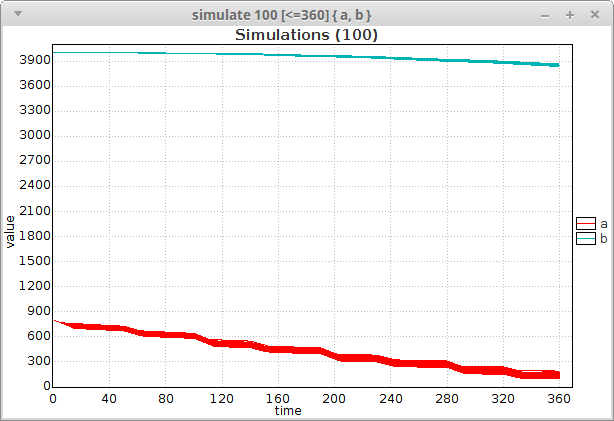
\includegraphics[width=0.60\textwidth]{graphics/ab.png}
		\end{figure}
\end{frame}

% Output 2
\begin{frame}[fragile]{Output}{Query 4.9}
	% query 4.9 - 
	\begin{equation*}
Pr\; [<=ScheduleLength] \; (<> \ skips \ !=\ 0)
	\end{equation*}
	% Result
	\begin{lstlisting}
Verifying formula 2 at line 2
-- Throughput: 64 states/sec, Load: 389 runs
-- Throughput: 386904 states/sec, Load: 389 runs
-- Throughput: 428461 states/sec, Load: 379 runs
-- Throughput: 427479 states/sec, Load: 367 runs
-- Throughput: 424452 states/sec, Load: 355 runs
-- Formula is satisfied.
(36 runs) Pr(<> ...) in [0,0.0973938]
with confidence 0.95.
	\end{lstlisting}
	\pause
	\begin{equation*}
		simulate\ 100 \; [<=ScheduleLength] \; \{active, \; Processor.Running\}
	\end{equation*}
\end{frame}

% Output 3
\begin{frame}[fragile]{Output}{Query 4.10}
	% query 4.10
	\begin{equation*}
		simulate\ 100 \; [<=ScheduleLength] \; \{active, \; Processor.Running\}
	\end{equation*}
	% Result
	\begin{lstlisting}
active:
[0]: (0,-1) (0.09,4) (13.828,4) (13.918,-1) ...
Processor.Running:
[0]: (0, 0) (0.09,1) (13.828,1) (13.918, 0) ...
	\end{lstlisting}
\end{frame}

% Output 3.1
\begin{frame}{Output}{Query 4.10}
	\begin{equation*}
		simulate\ 1 \; [<=ScheduleLength] \; \{active, \; Processor.Running\}
	\end{equation*}
	\begin{figure} % -1 og -2 IKKE 0 og 1 for .Running
		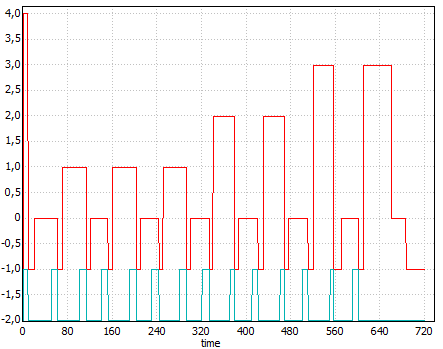
\includegraphics[width=0.45\textwidth]{graphics/activeprocessor.png}
		\end{figure}
\end{frame}

% Reflection 1 - batteri
\begin{frame}{Reflection}{Battery considerations}
	The battery is not a concern
	\begin{block}{Personal meeting with GomSpace, Lars Alminde}
		Not as important, more focus on clusters of satellites
	\end{block}
	Reasons:
	\begin{itemize}
		\item Greater battery capacity
		\item More efficient solar panels
	\end{itemize}
\end{frame}

% Reflection 2 - Robusthed
\begin{frame}{Reflection}{Robustness}
	Minimal functionality
	\begin{itemize}
		\item Varying time on payloads
	\end{itemize}
	Wanted functionality
	\begin{itemize}
		\item Randomly forced reboots
		\item Lessen the efficiently of the solar panels
		\item Payloads that takes longer than expected
	\end{itemize}
\end{frame}

\section{Battery Models and Robustness}
\subsection{Kinetic Battery Model}

\begin{frame}[fragile]{Battery Models}{\insertsubsection}
	\centering
	\begin{equation*}
	\begin{aligned}
		y_1(t) &= c*C*e^{-k't}+\frac{(C*k'c-I)(1-e^{-k't})}{k'}-\frac{I*c(k't-1+e^{-k't})}{k'}\\
		y_2(t) &= (1-c)C*e^{-k't}+C(1-c)(1-e^{-k't})-\frac{I(1-c)(k't-1+e^{-k't})}{k'}\\
		a '&== -i+k*(b/(1-c)-a/c)\\
		b '&== -k*(b/(1-c)-a/c)+(insolation*RechargeRate)
	\end{aligned}
	\end{equation*}
\end{frame}

\begin{frame}[fragile]{Battery Models}{\insertsubsection}
	\centering
	\begin{figure}[h]
		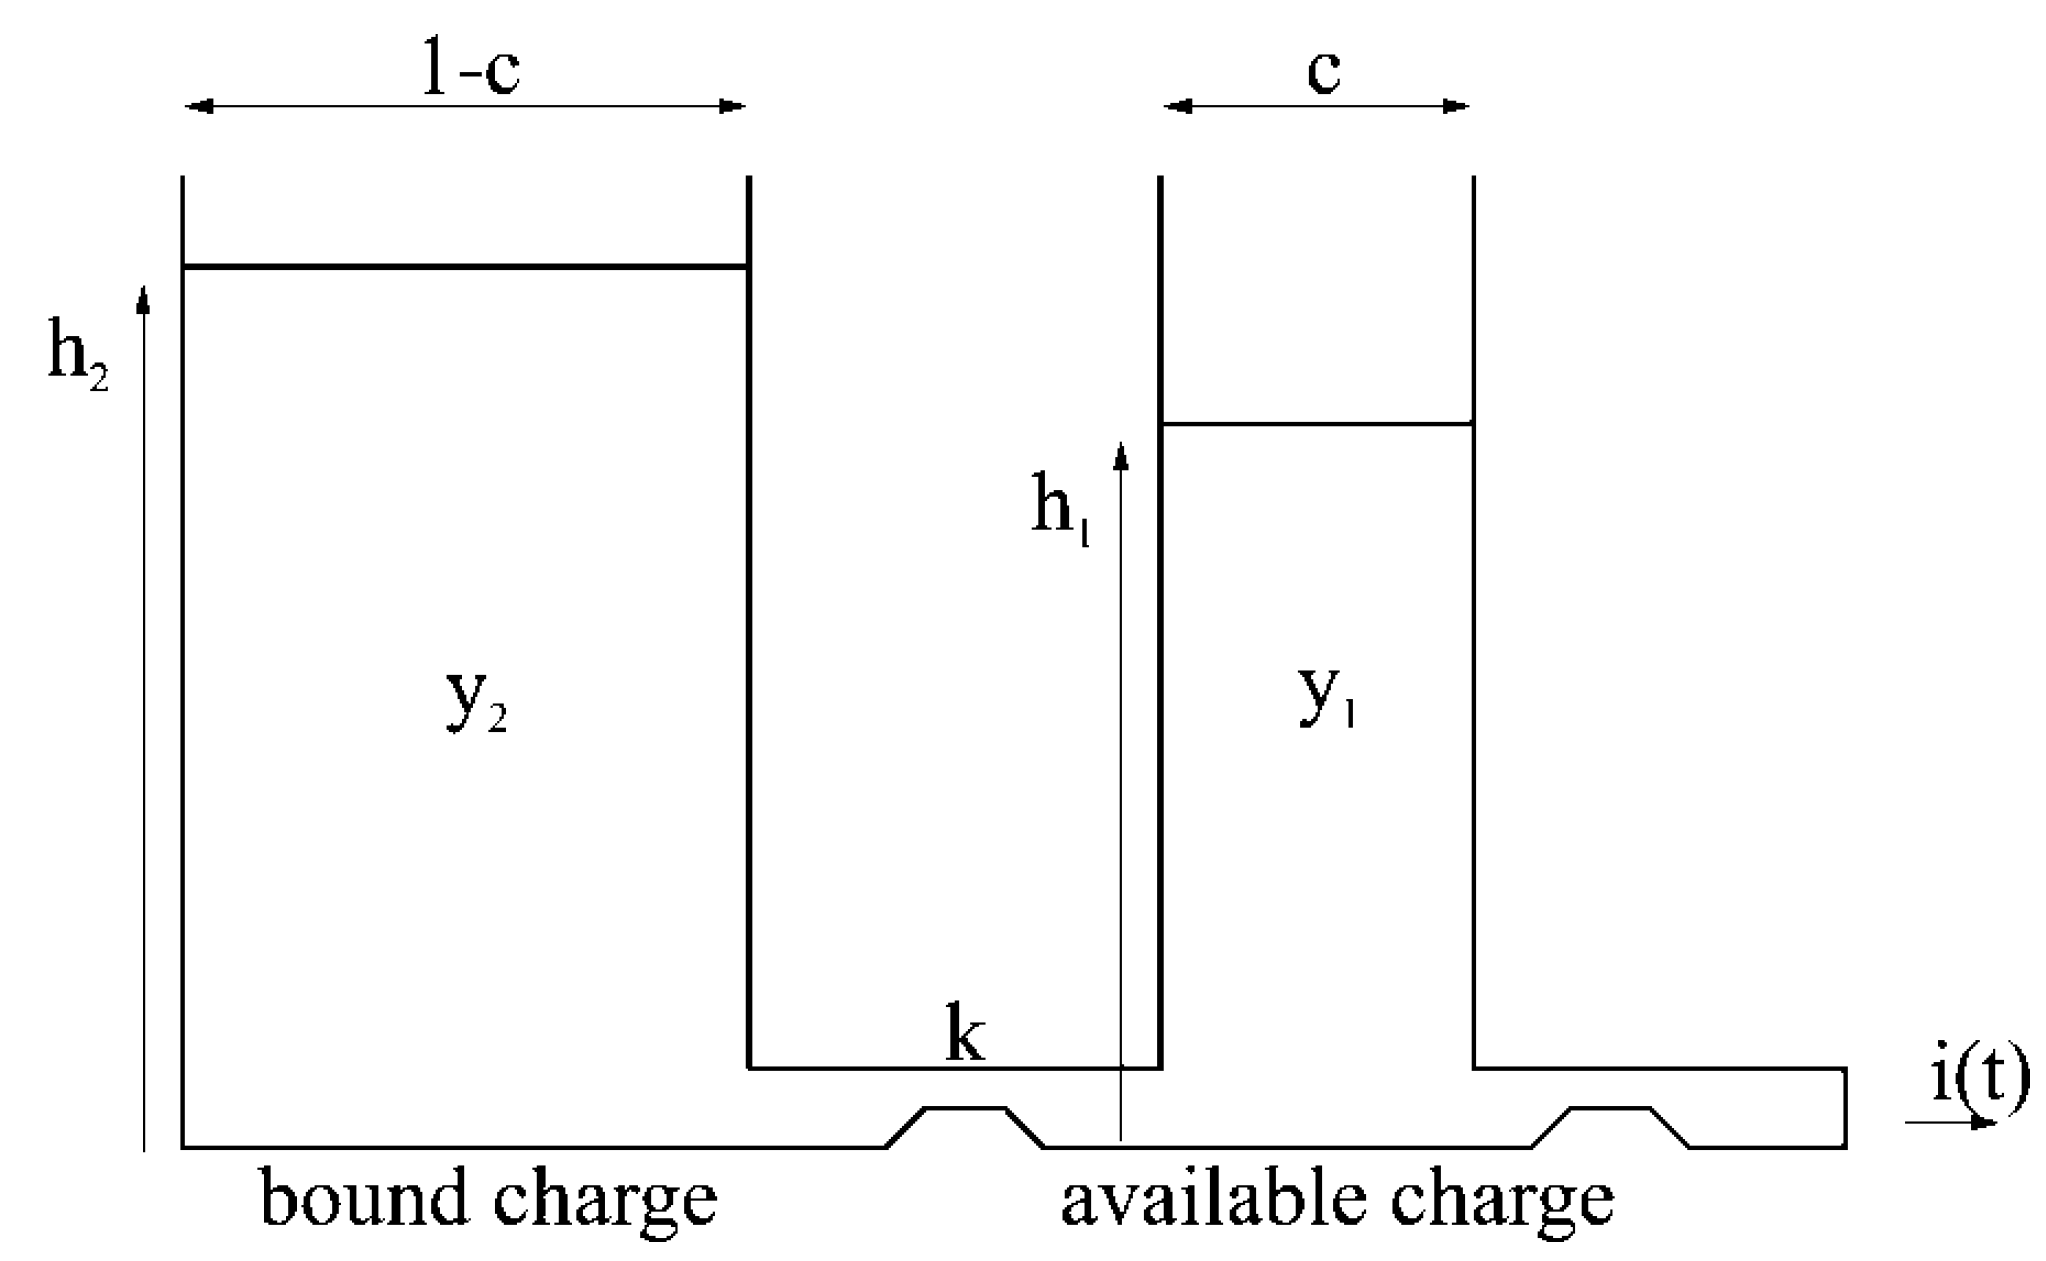
\includegraphics[width=.7\textwidth]{graphics/kibam_wells}
	\end{figure}
	\begin{equation*}
	\begin{aligned}
		y_1(t) &= c*C*e^{-k't}+\frac{(C*k'c-I)(1-e^{-k't})}{k'}-\frac{I*c(k't-1+e^{-k't})}{k'}\\
		y_2(t) &= (1-c)C*e^{-k't}+C(1-c)(1-e^{-k't})-\frac{I(1-c)(k't-1+e^{-k't})}{k'}
	\end{aligned}
	\end{equation*}
\end{frame}
\note{e growth, rate of change (compound interest)}
\begin{frame}[fragile]{Battery Models}{\insertsubsection}
	\centering
	\begin{figure}[h]
		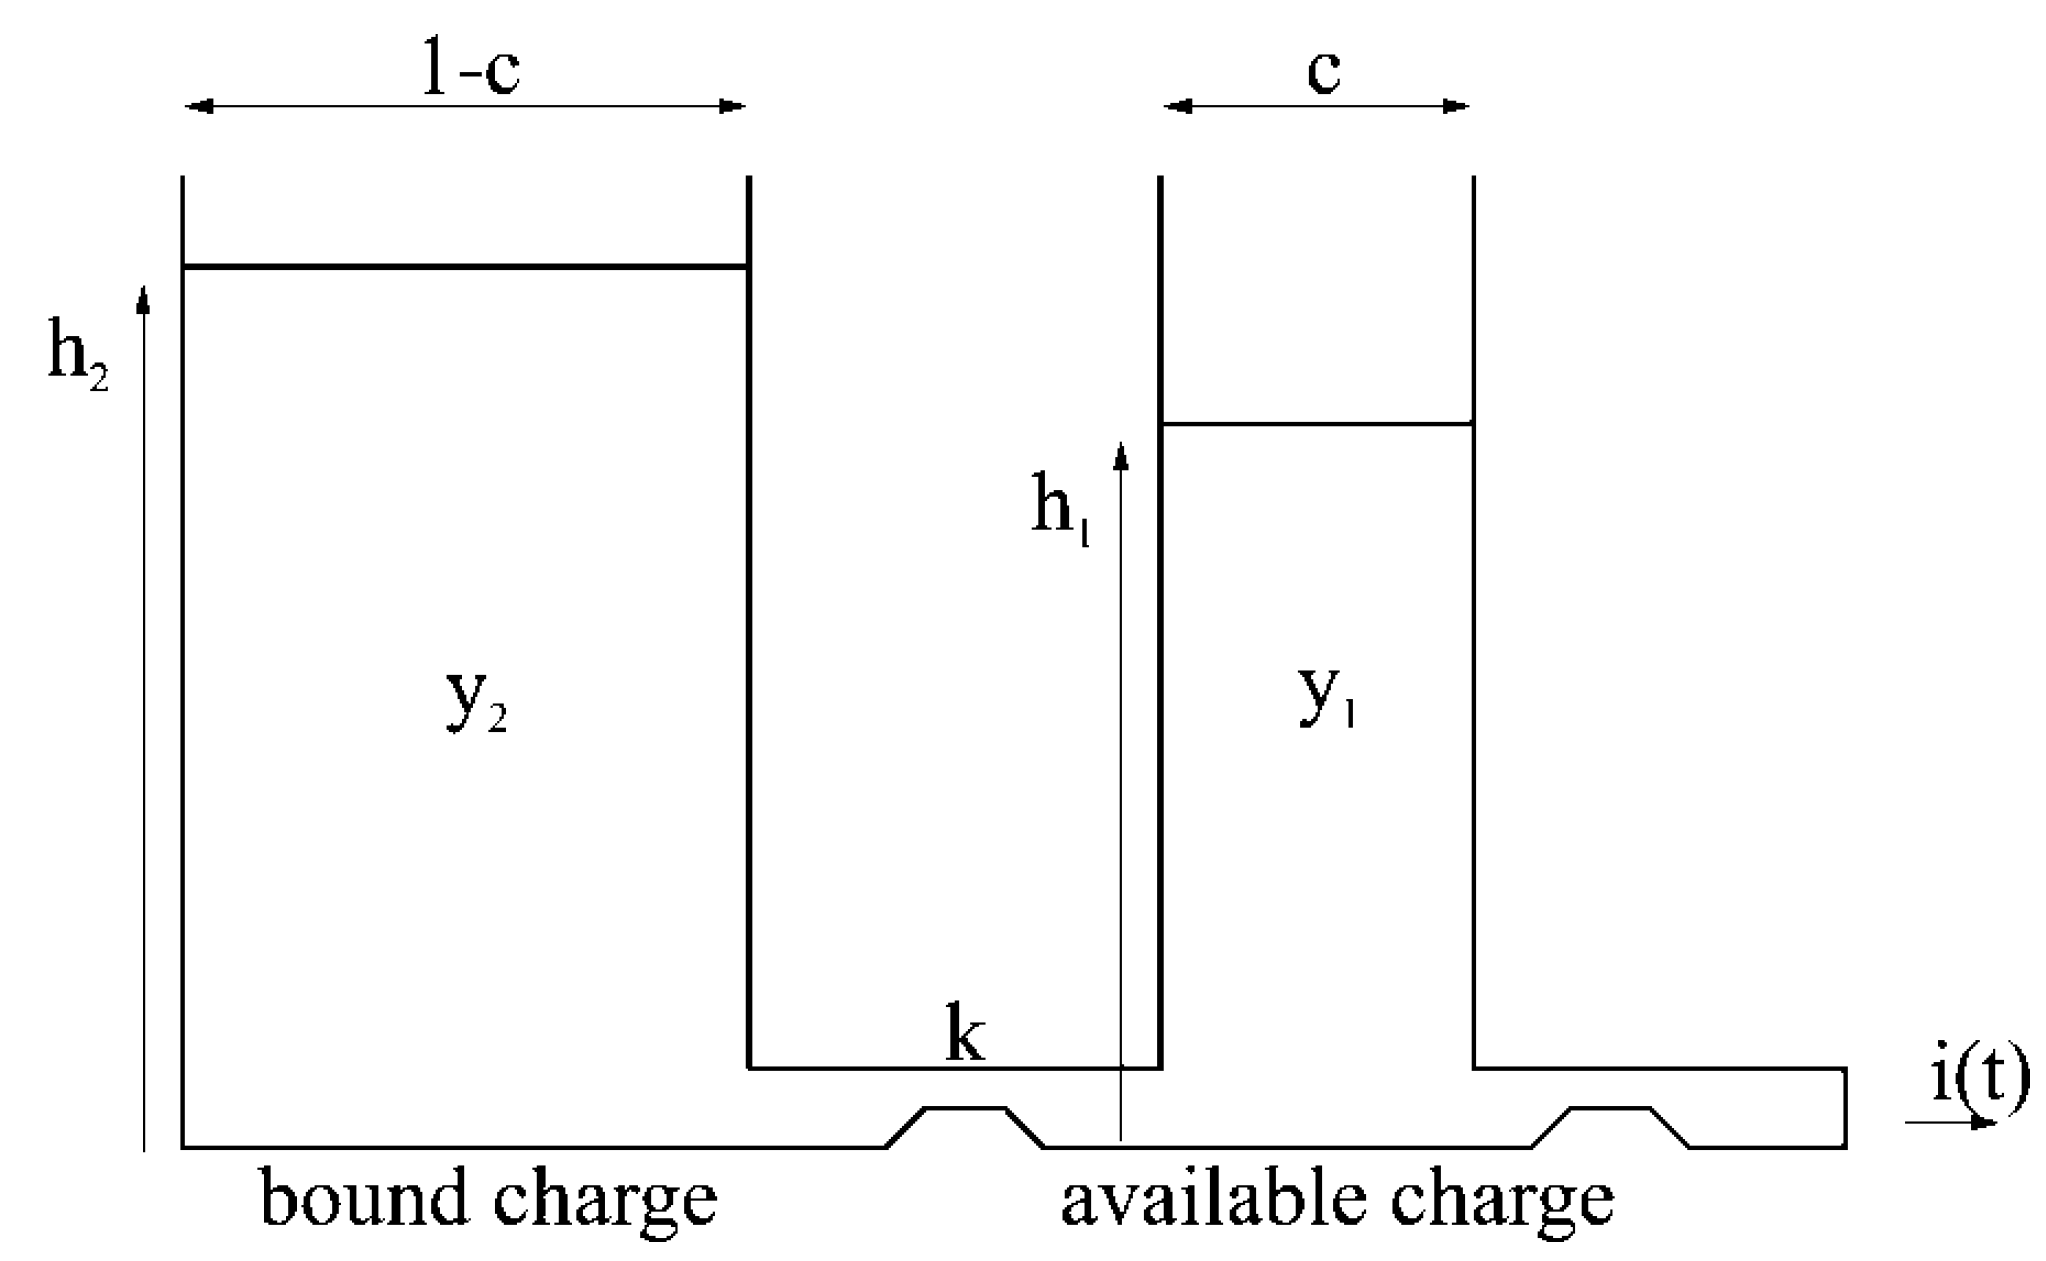
\includegraphics[width=.7\textwidth]{graphics/kibam_wells}
	\end{figure}
	\begin{equation*}
	\begin{aligned}
		\frac{dy_1}{dt} &= -i(t)+k(h_2-h_1)\\
		\frac{dy_2}{dt} &= -k(h_2-h_1)
	\end{aligned}
	\end{equation*}
\end{frame}

\begin{frame}[fragile]{Battery Models}{\insertsubsection}
	Calculate height of $h_1$ and $h_2$
	\begin{equation*}
	\begin{aligned}
		h_1 &= y_1/c\\
		h_2 &= y_2/1-c\\
		\frac{dy_1}{dt} &= -i(t)+k(h_2-h_1)\\
		\xrightarrow[dt]{} dy_1 &= -i+k(h_2-h_1) \\
		\xrightarrow[h_1, h_2]{} dy_1 &= -i+k(y_2/(1-c)-y_1/c)\\
		\xrightarrow[y_1, y_2]{} da &= -i+k(b/(1-c)-a/c)\\
		a '&== -i+k(b/(1-c)-a/c)
	\end{aligned}
	\end{equation*}
\end{frame}

\begin{frame}[fragile]{Battery Models}{\insertsubsection}
	\begin{equation*}
	\begin{aligned}
		db &= -k(b/1-c-a/c)\\
		b '&== -k*(b/(1-c)-a/c)+(insolation*RechargeRate)
	\end{aligned}
	\end{equation*}
	\begin{figure}[h]
		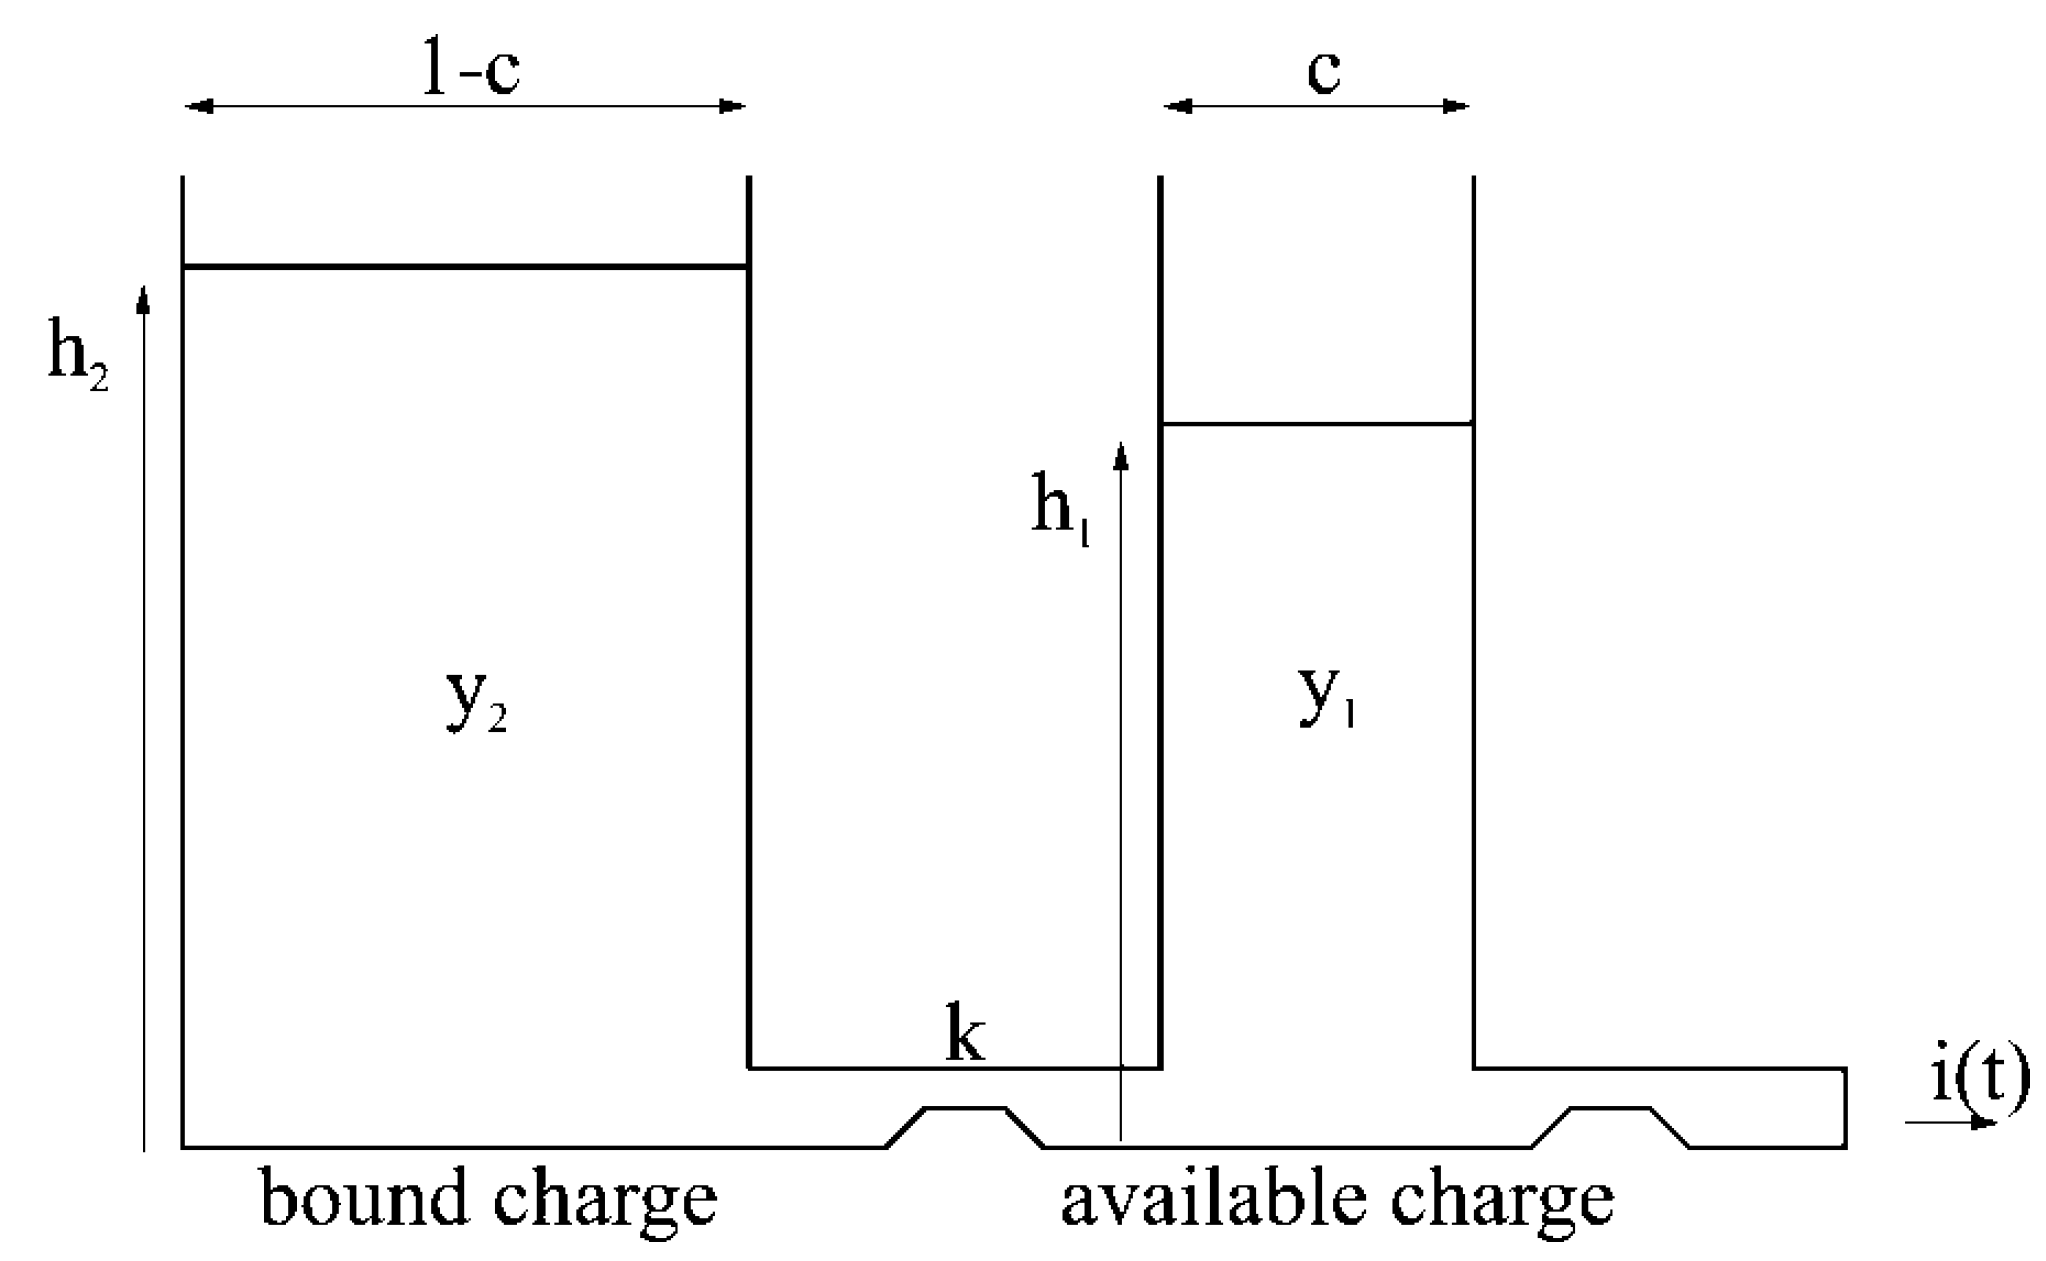
\includegraphics[width=.7\textwidth]{graphics/kibam_wells}
	\end{figure}
\end{frame}
\note{Talk about the inaccuarcy, we recharged energy is added to bound charge}

\subsection{Chose of Battery Model}
\begin{frame}[fragile]{Battery Models}{\insertsubsection}
\begin{table}[]
	\centering
	\begin{tabular}{lllll}
		\multicolumn{5}{c}{Variable load} \\
		\rowcolor[HTML]{EFEFEF} 
		Test & Meas, min & \%$\Delta$ Ideal & \%$\Delta$ Peukert & \%$\Delta$ KiBaM \\
		C1 & 54.5 & 29.91\% & 11.01\% & -33.39\% \\
		\rowcolor[HTML]{EFEFEF} 
		C2 & 73.3 & 25.38\% & 7.91\% & -24.01\% \\
		C3 & 88.3 & 22.88\% & 6.23\% & -19.14\% \\
		\rowcolor[HTML]{EFEFEF} 
		C4 & 136.0 & 19.85\% & 4.78\% & -9.12\% \\
		C5 & 182.7 & 18.50\% & 4.11\% & -3.83\% \\
		\rowcolor[HTML]{EFEFEF} 
		C6 & 59.0 & 26.61\% & 9.15\% & -30.34\% \\
		C7 & 51.1 & 30.92\% & 10.57\% & -40.31\% \\
		\rowcolor[HTML]{EFEFEF} 
		C8 & 55.0 & 28.73\% & 10.00\% & -30.73\% \\
		C9 & 54.9 & 28.96\% & 10.20\% & -36.61\% \\
		\rowcolor[HTML]{EFEFEF} 
		C10 & 142.7 & 20.04\% & 4.27\% & -7.71\%
	\end{tabular}
\end{table}
\end{frame}

\subsection{Functions and Variables}
\begin{frame}[fragile]{Robustness}{\insertsubsection}
	\centering
	\begin{figure}[h]
		
\includegraphics[width=1\textwidth]{graphics/payload_execution}
	\end{figure}
	\begin{figure}[h]
		\begin{minipage}{.7\textwidth}
		\begin{lstlisting}
N = 2;
Payloads[N][3] = {{10,15,20}, {7,15,20};
RunStart[NumberOfPayloads] = {50,100};
		\end{lstlisting}
		\end{minipage}\\
		\begin{minipage}{.7\textwidth}
			\begin{lstlisting}
void enqueue(){
	i = IIdle + Costs[active];
	B = Payloads[active][0];
	W = Payloads[active][1];
}
			\end{lstlisting}
		\end{minipage}
	\end{figure}
\end{frame}

\subsection{Processor Template}
\begin{frame}[fragile]{Robustness}{\insertsubsection}
\begin{figure}[H]
	\centering
	\begin{figure}[h]
		
\includegraphics[width=.8\textwidth]{graphics/payload_execution}
	\end{figure}\quad
	\scalebox{.6}{
	\begin{tikzpicture}
	%Locations
	\node [init] (l0) [label={[align=left]above:\textcolor{name}{Init}}] {$\cup$};
	\node [location] (l1) [right of=l0, xshift=40mm, label={
		[align=left]above:
		\textcolor{name}{Idle}},
	label={
		[align=center]below:
		\textcolor{invariant}{totalTime <= RunStart[payloadNumber]}
	}] {};
	\node [location] (l2) [right of=l1, xshift=80mm, label={
		[align=left]above:
		\textcolor{name}{Ready}
	}] {};
	\node [location] (l3) [below of=l0, yshift=-40mm, label={
		[align=left]below:
		\textcolor{name}{Done}
	}] {};
	\node [location] (l4) [below of=l1, yshift=-40mm, label={
		[align=left]below:
		\textcolor{name}{Wait}\\
		\textcolor{invariant}{x <= D}
	}] {};
	\node [location] (l5) [below of=l2, yshift=-40mm, label={
		[align=left]below:
		\textcolor{name}{Running}\\
		\textcolor{invariant}{x <= W}
	}] {};
	\path[->,black, thick] (l0) edge node [midway, above][align=left]{
		\textcolor{update}{t=0,i = IIdle,}\\
		\textcolor{update}{setActive()}} (l1);
	\path[->,black, thick] (l1) edge node [midway, above][align=center]{
		\textcolor{guard}{totalTime >=RunStart[payloadNumber]}\\
		\textcolor{sync}{ready!}\\
		\textcolor{update}{x=0, t=0,}\\
		\textcolor{update}{deadline()}} (l2);
	\path[->,black, thick] (l2) edge node [midway, right][align=left]{
		\textcolor{sync}{run?}\\
		\textcolor{update}{x := 0,}\\
		\textcolor{update}{setActive(),}\\
		\textcolor{update}{enqueue()}\\
		\textcolor{update}{earnings +=}\\
		\textcolor{update}{Profit[active]}} (l5);
	\path[->,black, thick] (l2) edge node [midway, left][align=left]{
		\textcolor{sync}{skip?}\\
		\textcolor{update}{payloadNumber ++,}\\
		\textcolor{update}{skipped()}} (l4);
	\path[->,black, thick] (l5) edge node [midway, below][align=left]{
		\textcolor{guard}{x >= B}\\
		\textcolor{update}{dequeue(), active = -1,}\\
		\textcolor{update}{payloadNumber ++}} (l4);
	\path[->,black, thick] (l4) edge node [midway, left][align=left]{
		\textcolor{guard}{x >= D \&\&}\\
		\textcolor{guard}{!done()}\\
		\textcolor{update}{setActive()}} (l1);
	\path[->,black, thick] (l4) edge node [midway, below][align=left]{
		\textcolor{guard}{done()}\\
		\textcolor{update}{on = false,}\\
		\textcolor{update}{active = -1}} (l3);
	\end{tikzpicture}}
	\caption{Processor template}
	\label{fig:smc_P}
\end{figure}
\end{frame}

\subsection{Queries}
\begin{frame}[fragile]{Robustness}{\insertsubsection}
	\centering
	
\end{frame}


\section{Section Three}
\begin{frame}[fragile]{\insertsection}{}
  \begin{itemize}
    \item item
    \begin{itemize}
      \item subitem
    \end{itemize}
    \item item
  \end{itemize}
\end{frame}

\subsection{Subsection Three}
\begin{frame}[fragile]{\insertsection with more text}{\insertsubsection}
  \begin{itemize}
    \item item
    \begin{itemize}
      \item subitem
    \end{itemize}
    \item item
  \end{itemize}
\end{frame}


%{\aauwavesbg
%\begin{frame}[plain,noframenumbering]
%\huge{Questions?}{}\\
%\includegraphics[width=0.75\textwidth]{graphics/metamoc.png}
%\end{frame}}

%\begin{frame}[plain,noframenumbering]
%\includegraphics[width=.90\textwidth]{graphics/upp.png}
%\end{frame}

\end{document}
